\clearpage
\section{Softwarearchitektur und Design}
\label{sec:software}

Die Software wird in C unter Linux auf beiden Raspberry Pis implementiert.
Threads werden verwendet, um Sensorerfassung, Kommunikation, Bedienung und
Safety-Logik voneinander zu trennen. Safety-relevante Entscheidungen werden auf
Raspberry Pi 2 getroffen; ein Ausfall von LCD oder Logging darf die
Motorabschaltung nicht verhindern.

\subsection{Raspberry Pi 1 -- Host und Bedienung}

\begin{table}[H]
    \centering
    \small
    \begin{tabularx}{\textwidth}{@{}p{4.2cm}Y@{}}
        \toprule
        \textbf{Modul / Thread} & \textbf{Aufgabe} \\
        \midrule
        Initialisierung & Bluetooth, LCD, Logging und benötigte Threads starten \\
        UI / Eingabe & Geschwindigkeitsstufe \texttt{LOW}, \texttt{MEDIUM}, \texttt{HIGH} auswählen und Programmende anfordern \\
        Kommunikations-/Heartbeat-Thread & Sollstufe und Heartbeat alle 100 ms senden; Status und Fehlermeldungen von Pi 2 empfangen \\
        Anzeige & Systemzustand, Geschwindigkeitsstufe, kleinsten gemessenen Abstand $d_{\min}$ und Fehlercode am LCD anzeigen (siehe Abschnitt~\ref{sec:distances}) \\
        Logging & Ereignisse sofort und Messwerte mit 10 Hz protokollieren (siehe Abschnitt~\ref{sec:logging}); keine Safety-Funktion \\
        \bottomrule
    \end{tabularx}
    \caption{Softwareaufgaben auf Raspberry Pi 1}
\end{table}

\subsection{Raspberry Pi 2 -- Steuerung und Überwachung}

\begin{table}[H]
    \centering
    \small
    \begin{tabularx}{\textwidth}{@{}p{4.2cm}Y@{}}
        \toprule
        \textbf{Modul / Thread} & \textbf{Aufgabe} \\
        \midrule
        Initialisierung & Motor sicher deaktivieren, Sensoren, Bluetooth und Threads initialisieren \\
        Sensor-Thread 1 / 2 & HC-SR04 auslesen; Messbereich und Abstandsänderung prüfen; Messwert, Gültigkeitsstatus und Zeitstempel bereitstellen \\
        Kommunikations-Thread & Nachrichten von Pi 1 empfangen und prüfen; Heartbeat-Timeout überwachen; Status alle 100 ms an Pi 1 senden \\
        Safety-Logik-Thread & Zyklisch alle 50 ms Sensorplausibilität, Kommunikation und Datenaktualität prüfen; Sicherheitsabstand auswählen und Motorfreigabe entscheiden \\
        Motorsteuerungs-Thread & Motorstufe setzen oder Motor mit PWM = 0 und Enable = OFF abschalten \\
        \bottomrule
    \end{tabularx}
    \caption{Softwareaufgaben auf Raspberry Pi 2}
\end{table}

\subsection{Safety-Logik-Thread}

Der Safety-Logik-Thread ist ein eigener Thread auf Raspberry Pi 2. Er führt
keine blockierenden Netzwerk- oder Logging-Aufrufe aus. In jedem Zyklus werden
folgende Prüfungen in dieser Reihenfolge ausgeführt:

\begin{enumerate}
    \item Wurde ein Stop/Shutdown-Befehl empfangen?
    \item Sind beide Sensorwerte gültig und zueinander plausibel?
    \item Ist die Kommunikation aktuell und der empfangene Befehl gültig?
    \item Sind die verwendeten Sensordaten noch aktuell?
    \item Welcher Sicherheitsabstand gehört zur gültigen Geschwindigkeitsstufe?
    \item Liegt der aktuelle Abstand innerhalb des Sicherheitsabstands?
\end{enumerate}

Wurde ein Stop/Shutdown-Befehl empfangen, wird der Motor abgeschaltet und das
Programm kontrolliert beendet. Schlägt eine der Prüfungen 2 bis 4 fehl, wird ein
Fehlerzustand gesetzt und die Motoransteuerung deaktiviert. Erst wenn alle Prüfungen erfolgreich sind,
darf die normale Motorsteuerung ausgeführt werden.

\subsection{Verwendete Abstände}
\label{sec:distances}

Die Abstandsüberwachung verwendet folgende Größen:

\begin{table}[H]
    \centering
    \small
    \begin{tabularx}{\textwidth}{@{}p{3.6cm}Y@{}}
        \toprule
        \textbf{Größe} & \textbf{Bedeutung} \\
        \midrule
        $d_1$, $d_2$ & Gemessene Abstände von Sensor 1 und Sensor 2. Beide werden benötigt, um die Sensoren gegeneinander zu prüfen (P3). \\
        $d_{\min} = \min(d_1, d_2)$ & Kleinerer der beiden gültigen Messwerte. Er wird für die Abschaltentscheidung verwendet, weil er den ungünstigeren Fall darstellt. \\
        $S_{\mathrm{LOW}}$, $S_{\mathrm{MEDIUM}}$, $S_{\mathrm{HIGH}}$ & Sicherheitsabstand je Geschwindigkeitsstufe. Bei höherer Stufe sind Nachlaufzeit und zurückgelegter Weg des Rotors größer, deshalb gilt $S_{\mathrm{LOW}} < S_{\mathrm{MEDIUM}} < S_{\mathrm{HIGH}}$. \\
        $S$ & Aktiver Sicherheitsabstand, also der Wert, der zur aktuell gültigen Geschwindigkeitsstufe gehört. Der Motor wird abgeschaltet, wenn $d_{\min} < S$. \\
        \bottomrule
    \end{tabularx}
    \caption{Begriffe der Abstandsüberwachung}
\end{table}

Am LCD wird nur $d_{\min}$ angezeigt. $d_1$ und $d_2$ werden einzeln
protokolliert, damit Abweichungen zwischen den Sensoren nachvollziehbar sind.

\subsection{Plausibilitätsprüfung der Sensorwerte}
\label{sec:plausibility}

Ein Sensorwert wird nur verwendet, wenn er die Prüfungen P1--P4 besteht. Die
Prüfungen P1 und P2 betreffen jeden Sensor einzeln und werden im jeweiligen
Sensor-Thread durchgeführt. Das Ergebnis wird als Gültigkeitsstatus im
Datensatz abgelegt. P3 und P4 vergleichen bzw. bewerten die Daten und werden im
Safety-Logik-Thread durchgeführt.

\begin{table}[H]
    \centering
    \small
    \begin{tabularx}{\textwidth}{@{}p{0.7cm}p{3.1cm}Yp{2.3cm}@{}}
        \toprule
        \textbf{ID} & \textbf{Prüfung} & \textbf{Bedingung für „ungültig“} & \textbf{Ort} \\
        \midrule
        P1 & Messbereich & $d < 2$ cm oder $d > 400$ cm (Grenzen des HC-SR04). Bleibt das Echo aus (Timeout), wird der Messwert ebenfalls als ungültig markiert. & Sensor-Thread \\
        P2 & Abstandsänderung & $\frac{|d_k - d_{k-1}|}{t_k - t_{k-1}} > 0{,}2$ cm/ms, also eine Änderung schneller als 2 m/s zwischen zwei Messungen desselben Sensors. & Sensor-Thread \\
        P3 & Quervergleich & $|d_1 - d_2| > 5$ cm in zwei aufeinanderfolgenden Messzyklen. & Safety-Logik \\
        P4 & Datenalter & Messwert älter als 150 ms. & Safety-Logik \\
        \bottomrule
    \end{tabularx}
    \caption{Plausibilitätsprüfungen der Abstandssensoren}
\end{table}

Die Grenze von 2 m/s in P2 entspricht der Annäherungsgeschwindigkeit, die die
EN ISO 13855 für Handbewegungen ansetzt. P2 filtert vor allem Ausreißer und
Sprünge des Messwerts. Taucht ein Objekt seitlich im Messbereich auf oder nähert
es sich schneller, kann der Messwert ebenfalls sprunghaft kleiner werden und P2
auslösen. Die Reaktion ist in allen Fällen Motor AUS und liegt damit auf der
sicheren Seite.

\subsection{Systemzustände}
\label{sec:states}

Raspberry Pi 2 befindet sich immer in genau einem der folgenden Zustände. Der
aktuelle Zustand wird im Status an Pi 1 übertragen und am LCD angezeigt.

\begin{table}[H]
    \centering
    \small
    \begin{tabularx}{\textwidth}{@{}p{2.7cm}p{2.2cm}Y@{}}
        \toprule
        \textbf{Zustand} & \textbf{Motor} & \textbf{Bedeutung} \\
        \midrule
        \texttt{INIT} & AUS & Programmstart; Schnittstellen und Threads werden initialisiert. Noch keine Safety-Bewertung. \\
        \texttt{BETRIEB} & AN (\texttt{LOW}, \texttt{MEDIUM} oder \texttt{HIGH}) & Alle Prüfungen bestanden und $d_{\min} \geq S$. \\
        \texttt{OBJEKT\_STOPP} & AUS & Alle Prüfungen bestanden, aber $d_{\min} < S$. Kein Fehler, sondern bestimmungsgemäße Schutzreaktion. \\
        \texttt{FEHLER} & AUS & Mindestens eine Prüfung fehlgeschlagen. Ein Fehlercode gibt die Ursache an: \texttt{SENSOR} (P1--P3), \texttt{KOMMUNIKATION} (Timeout oder ungültiger Befehl), \texttt{DATENALTER} (P4). \\
        \texttt{SHUTDOWN} & AUS & Stop/Shutdown-Befehl empfangen; Threads werden kontrolliert beendet. Endzustand. \\
        \bottomrule
    \end{tabularx}
    \caption{Systemzustände von Raspberry Pi 2}
\end{table}

\texttt{INIT} wird nach Abschluss der Initialisierung verlassen. Danach wird der
Zustand in jedem Zyklus des Safety-Logik-Threads neu aus den Prüfergebnissen
bestimmt, in derselben Reihenfolge wie im Flussdiagramm
(Abbildung~\ref{fig:flowchart}):

\begin{enumerate}
    \item Stop/Shutdown empfangen $\rightarrow$ \texttt{SHUTDOWN}
    \item Eine der Prüfungen Sensorplausibilität, Kommunikation oder Datenaktualität fehlgeschlagen $\rightarrow$ \texttt{FEHLER}
    \item $d_{\min} < S$ $\rightarrow$ \texttt{OBJEKT\_STOPP}
    \item sonst $\rightarrow$ \texttt{BETRIEB}
\end{enumerate}

\textbf{Wiederanlaufbedingung:} Der Zustand \texttt{FEHLER} ist nicht selbsthaltend. Aus
\texttt{FEHLER} oder \texttt{OBJEKT\_STOPP} geht das System in \texttt{BETRIEB}
über, sobald in einem Zyklus alle folgenden Bedingungen gleichzeitig erfüllt
sind:

\begin{itemize}
    \item kein Stop/Shutdown-Befehl empfangen,
    \item beide Sensorwerte gültig und zueinander plausibel (P1--P3),
    \item gültige Nachricht von Pi 1 innerhalb der letzten 300 ms mit gültiger Geschwindigkeitsstufe,
    \item Sensordaten nicht älter als 150 ms (P4),
    \item $d_{\min} \geq S$ für die aktuell gültige Stufe.
\end{itemize}

Die Motorstufe wird dann im selben Zyklus freigegeben, und der Motor läuft mit
der von Pi 1 angeforderten Stufe an. Eine Quittierung durch den Bediener
ist nicht vorgesehen; die daraus folgenden Einschränkungen sind in
Abschnitt~\ref{sec:limits} beschrieben.

Auf Pi 1 wird zusätzlich „Verbindung getrennt“ angezeigt, wenn länger
als 300 ms kein gültiger Status von Pi 2 empfangen wurde. Der zuletzt
empfangene Zustand wird dann nicht mehr als aktuell dargestellt.

\subsection{Gemeinsam verwendete Daten}
\label{sec:shared}

Sensor- und Kommunikations-Threads aktualisieren Daten, die vom
Safety-Logik-Thread gelesen werden. Damit keine Race Conditions entstehen,
werden zusammengehörige Werte als Datensatz behandelt, zum Beispiel:

\begin{verbatim}
struct sensor_data {
    float distance_cm;
    bool valid;
    struct timespec timestamp;
};
\end{verbatim}

Der schreibende Thread aktualisiert den vollständigen Datensatz geschützt durch
einen Mutex. Der Safety-Logik-Thread kopiert den Datensatz unter demselben Mutex
in eine lokale Variable und arbeitet anschließend nur mit diesem Snapshot.
Zeitmessungen für Timeouts und Datenalter erfolgen mit der monotonen Uhr
\texttt{CLOCK\_MONOTONIC} (siehe Abschnitt~\ref{subsec:security-addressed}, T3).

Konkret werden folgende gemeinsamen Datensätze verwendet:

\begin{table}[H]
    \centering
    \small
    \begin{tabularx}{\textwidth}{@{}p{3.2cm}p{3.0cm}p{3.0cm}Y@{}}
        \toprule
        \textbf{Datensatz} & \textbf{Schreibt} & \textbf{Liest} & \textbf{Inhalt} \\
        \midrule
        \texttt{sensor\_data[2]} & Sensor-Thread 1 / 2 & Safety-Logik, Kommunikation & Abstand, Gültigkeit (P1, P2), Zeitstempel \\
        \texttt{comm\_data} & Kommunikations-Thread & Safety-Logik & Sollstufe, Stop-Flag, Zeitstempel der letzten gültigen Nachricht \\
        \texttt{safety\_state} & Safety-Logik & Kommunikation, Motorsteuerung & Systemzustand, Fehlercode, freigegebene Motorstufe \\
        \bottomrule
    \end{tabularx}
    \caption{Gemeinsame Datensätze auf Raspberry Pi 2}
\end{table}

Für die Umsetzung gelten folgende Regeln:

\begin{itemize}
    \item Jeder Datensatz hat genau einen schreibenden Thread und einen eigenen \texttt{pthread\_mutex\_t}.
    \item Die Mutexe werden mit dem Protokoll \texttt{PTHREAD\_PRIO\_INHERIT} angelegt, damit ein niedriger priorisierter Thread den Safety-Logik-Thread nicht durch Prioritätsinversion aufhält.
    \item Unter einem Mutex wird nur kopiert. Messungen, Bluetooth-Zugriffe, Logging und GPIO-Zugriffe erfolgen außerhalb des gesperrten Bereichs.
    \item Ein Thread hält immer nur einen Mutex gleichzeitig; dadurch sind Deadlocks ausgeschlossen.
    \item Der Safety-Logik-Thread läuft mit \texttt{SCHED\_FIFO} und der höchsten Priorität der Anwendung.
    \item Nur der Safety-Logik-Thread schreibt die freigegebene Motorstufe. Die Motorsteuerung setzt ausschließlich diesen Wert um.
\end{itemize}

\subsection{Bluetooth-Kommunikation}
\label{sec:bt}

Die Kommunikation ist bidirektional. Raspberry Pi 1 sendet Sollstufe,
Heartbeat, Sequenznummer und gegebenenfalls einen Stop/Shutdown-Befehl.
Raspberry Pi 2 sendet Status, aktuelle Abstandswerte und Fehlermeldungen zurück.

Bevor die Nutzdaten gelesen werden, prüft Pi 2, ob die Länge zum
Nachrichtentyp passt. Ein unbekannter Typ oder eine falsche Länge führt zum
Abbau der Verbindung, da der Datenstrom danach nicht mehr synchron ist. Nach dem
Einlesen prüft Pi 2 zuerst das GCM-Tag, danach Session-ID, Sequenznummer und
Wertebereich der Nutzdaten. Schlägt eine dieser Prüfungen fehl, wird die
Nachricht verworfen. Bleibt eine gültige Nachricht länger als
300 ms aus, wird die Kommunikation als fehlerhaft bewertet und der Motor
abgeschaltet.

\textbf{Umsetzung der Datenübertragung:}

\begin{itemize}
    \item Die Verbindung wird als RFCOMM-Socket über die BlueZ-Socket-API aufgebaut (\texttt{AF\_BLUETOOTH}, \texttt{SOCK\_STREAM}, \texttt{BTPROTO\_RFCOMM}). Pi 2 ist Server und wartet auf einem festen Kanal, Pi 1 ist Client. Die beiden Geräte werden einmalig gekoppelt. Nach dem Verbindungsaufbau sendet Pi 2 zuerst eine \texttt{STATUS}-Nachricht mit einer neuen Session-ID; erst danach beginnt Pi 1 mit den Heartbeats (siehe Abschnitt~\ref{subsec:security-addressed}, T2).
    \item Da RFCOMM einen Datenstrom und keine einzelnen Pakete liefert, beginnt jede Nachricht mit einem Typ- und einem Längenfeld. Der Empfänger liest zuerst diese Felder und danach genau die angegebene Anzahl Bytes.
    \item Nachrichten werden Feld für Feld in ein Byte-Array in Big-Endian-Reihenfolge (Network Byte Order, umgesetzt mit \texttt{htons()} und \texttt{htonl()}) geschrieben, nicht als C-\texttt{struct} kopiert. Dadurch spielen Padding und Compiler-Unterschiede keine Rolle.
    \item Abstände werden als ganze Millimeter (\texttt{uint16\_t}) übertragen, Stufen, Zustände und Fehlercodes als \texttt{uint8\_t} mit festgelegten Werten. Unbekannte Werte führen zum Verwerfen der Nachricht.
    \item Der Kommunikations-Thread wartet mit \texttt{poll()} und einem Timeout von 50 ms auf Daten. Er blockiert dadurch nie dauerhaft und kann den Heartbeat-Timeout auch dann auswerten, wenn keine Daten ankommen.
    \item Bricht die Verbindung ab, versucht Pi 1 jede Sekunde, sie neu aufzubauen. Pi 2 bleibt währenddessen über den Kommunikations-Timeout im Zustand \texttt{FEHLER}.
\end{itemize}

\begin{table}[H]
    \centering
    \small
    \begin{tabularx}{\textwidth}{@{}p{2.6cm}p{2.3cm}p{2.0cm}Y@{}}
        \toprule
        \textbf{Nachricht} & \textbf{Richtung} & \textbf{Takt} & \textbf{Nutzdaten} \\
        \midrule
        \texttt{HEARTBEAT} & Pi 1 $\rightarrow$ Pi 2 & 100 ms & Sollstufe \\
        \texttt{STOP} & Pi 1 $\rightarrow$ Pi 2 & bei Bedarf & -- \\
        \texttt{STATUS} & Pi 2 $\rightarrow$ Pi 1 & 100 ms & Systemzustand, Fehlercode, aktive Stufe, $d_1$, $d_2$ \\
        \texttt{ACK} & Pi 2 $\rightarrow$ Pi 1 & bei Bedarf & Bestätigung des kontrollierten Shutdowns \\
        \bottomrule
    \end{tabularx}
    \caption{Nachrichtentypen zwischen Pi 1 und Pi 2}
\end{table}

Tabelle~\ref{tab:frame} zeigt den Aufbau eines Frames,
Tabelle~\ref{tab:kodierung} die Kodierung der Werte. Die kryptografische
Absicherung ist in Abschnitt~\ref{subsec:security-addressed} (T1, T2)
beschrieben.

\begin{table}[H]
    \centering
    \small
    \begin{tabularx}{\textwidth}{@{}p{1.3cm}p{3.0cm}p{1.4cm}Y@{}}
        \toprule
        \textbf{Offset} & \textbf{Feld} & \textbf{Größe} & \textbf{Inhalt} \\
        \midrule
        0 & Typ & 1 B & Nachrichtentyp (Tabelle~\ref{tab:kodierung}) \\
        1 & Länge & 2 B & Länge $n$ der Nutzdaten in Byte \\
        3 & Session-ID & 4 B & Zufallswert von Pi 2 je Verbindung \\
        7 & Sequenznummer & 4 B & beginnt je Verbindung bei 1 \\
        11 & Nonce & 12 B & zufällig je Nachricht (\texttt{getrandom()}) \\
        23 & Nutzdaten & $n$ B & mit AES-256-GCM verschlüsselt \\
        $23+n$ & Tag & 16 B & GCM-Authentifizierungstag \\
        \bottomrule
    \end{tabularx}
    \caption{Aufbau eines Frames. Die Bytes 0--10 (Typ, Länge, Session-ID,
    Sequenznummer) werden unverschlüsselt übertragen und als AAD authentifiziert.}
    \label{tab:frame}
\end{table}

\begin{table}[H]
    \centering
    \small
    \begin{tabularx}{\textwidth}{@{}p{2.2cm}Y@{}}
        \toprule
        \textbf{Feld} & \textbf{Kodierung (\texttt{uint8\_t}, sofern nicht anders angegeben)} \\
        \midrule
        Typ & \texttt{0x01} \texttt{HEARTBEAT} ($n=1$), \texttt{0x02} \texttt{STOP} ($n=0$), \texttt{0x03} \texttt{STATUS} ($n=7$), \texttt{0x04} \texttt{ACK} ($n=0$) \\
        Stufe & \texttt{0x01} \texttt{LOW}, \texttt{0x02} \texttt{MEDIUM}, \texttt{0x03} \texttt{HIGH}; in \texttt{STATUS} zusätzlich \texttt{0x00} = Motor AUS \\
        Zustand & \texttt{0x00} \texttt{INIT}, \texttt{0x01} \texttt{BETRIEB}, \texttt{0x02} \texttt{OBJEKT\_STOPP}, \texttt{0x03} \texttt{FEHLER}, \texttt{0x04} \texttt{SHUTDOWN} \\
        Fehlercode & \texttt{0x00} kein Fehler, \texttt{0x01} \texttt{SENSOR}, \texttt{0x02} \texttt{KOMMUNIKATION}, \texttt{0x03} \texttt{DATENALTER} \\
        $d_1$, $d_2$ & \texttt{uint16\_t} in mm; \texttt{0xFFFF} = kein gültiger Messwert \\
        \bottomrule
    \end{tabularx}
    \caption{Kodierung der Nutzdaten. \texttt{HEARTBEAT} enthält die Sollstufe;
    \texttt{STATUS} enthält Zustand, Fehlercode, aktive Stufe, $d_1$ und $d_2$ in
    dieser Reihenfolge.}
    \label{tab:kodierung}
\end{table}

\subsection{Motorsteuerung}

Die Motorsteuerung erhält ausschließlich eine bereits durch die Safety-Logik
freigegebene Geschwindigkeitsstufe. Eine unbekannte oder ungültige Stufe führt
nicht zu einem Default-Betrieb, sondern zu Motor AUS. Der sichere Softwarezustand
wird durch

\begin{center}
    \texttt{PWM = 0} und \texttt{Enable = OFF}
\end{center}

angefordert. \texttt{Enable} bezeichnet dabei den Standby-Eingang STBY des
Motortreibers TB6612FNG; \texttt{Enable = OFF} entspricht STBY = LOW. Der
mechanische Nachlauf des Rotors wird dadurch nicht aufgehoben.

\subsection{Anzeige und Logging}
\label{sec:logging}

Anzeige und Logging laufen auf Pi 1 und sind keine Safety-Funktionen. Das LCD
zeigt Systemzustand, Geschwindigkeitsstufe, $d_{\min}$ und gegebenenfalls den
Fehlercode an und wird bei jedem empfangenen Status aktualisiert.

Protokolliert wird auf zwei Arten:

\begin{itemize}
    \item \textbf{Ereignisse} werden sofort beim Auftreten protokolliert: Zustandswechsel, neuer Fehlercode, Änderung der Sollstufe durch den Bediener, Verbindungsverlust und Wiederaufbau, Programmstart und Stop/Shutdown.
    \item \textbf{Messwerte} werden mit 10 Hz protokolliert, also bei jeder empfangenen \texttt{STATUS}-Nachricht: Zeitstempel, Zustand, Fehlercode, Stufe, $d_1$ und $d_2$.
\end{itemize}

Das Log wird als CSV-Datei geschrieben. Die Ausgabe erfolgt gepuffert und wird
einmal pro Sekunde sowie bei jedem Fehlerereignis auf die SD-Karte
geschrieben, damit Logging die Bedienung und Kommunikation nicht verzögert.

Im Testmodus protokolliert Pi 2 zusätzlich den Empfangszeitpunkt der letzten
gültigen Nachricht und den Zeitpunkt jedes Zustandswechsels mit seiner monotonen
Uhr in eine lokale Datei, um Reaktionszeiten messen zu können. Die Datei wird
außerhalb des Safety-Logik-Threads geschrieben.

\subsection{Initialisierung und kontrolliertes Beenden}

Beim Start von Raspberry Pi 2 ist die Motoransteuerung deaktiviert. Eine
Motorfreigabe ist erst erlaubt, wenn Initialisierung, Sensorprüfung und
Kommunikationsprüfung erfolgreich abgeschlossen wurden.

Fordert der Benutzer auf Raspberry Pi 1 das Programmende an, sendet Pi 1 einen
Stop/Shutdown-Befehl. Pi 2 setzt zuerst den Motor in den sicheren Zustand,
beendet danach seine Threads und schließt die Bluetooth-Verbindung. Anschließend
kann Pi 1 seine eigenen Threads und Ressourcen kontrolliert beenden.

\subsection{Programmierrichtlinien und Versionskontrolle}

Der C-Code orientiert sich an MISRA~C. Die Einhaltung wird mit cppcheck und
dessen MISRA-Addon geprüft; bewusste Abweichungen werden im Code begründet.
Insbesondere werden feste Datentypen, geprüfte Rückgabewerte, definierte
Wertebereiche, ein \texttt{default}-Zweig in \texttt{switch}-Anweisungen und
möglichst kurze, klar abgegrenzte Funktionen verwendet. Gemeinsame Konstanten
wie Timeouts und Grenzwerte werden zentral definiert.

Das gesamte Projekt wird mit Git versioniert. Im
Repository liegen:

\begin{itemize}
    \item der Quellcode von Pi 1 und Pi 2,
    \item gemeinsame Header-Dateien (Nachrichtenformat, Konstanten und Grenzwerte),
    \item Build-Dateien und Testskripte,
    \item dieses Designdokument.
\end{itemize}

Ausgenommen ist nur das kryptografische Schlüsselmaterial, das über
\texttt{.gitignore} vom Repository ausgeschlossen wird. Änderungen am
Safety-relevanten Code auf Pi 2 werden über einen Pull Request eingebracht und
vor dem Merge von einem zweiten Gruppenmitglied geprüft.

\clearpage
\subsection{Pinout}
\label{sec:pinout}

Die folgenden Abbildungen zeigen die Pinbelegung der beiden Raspberry Pis.

\begin{figure}[H]
    \centering
    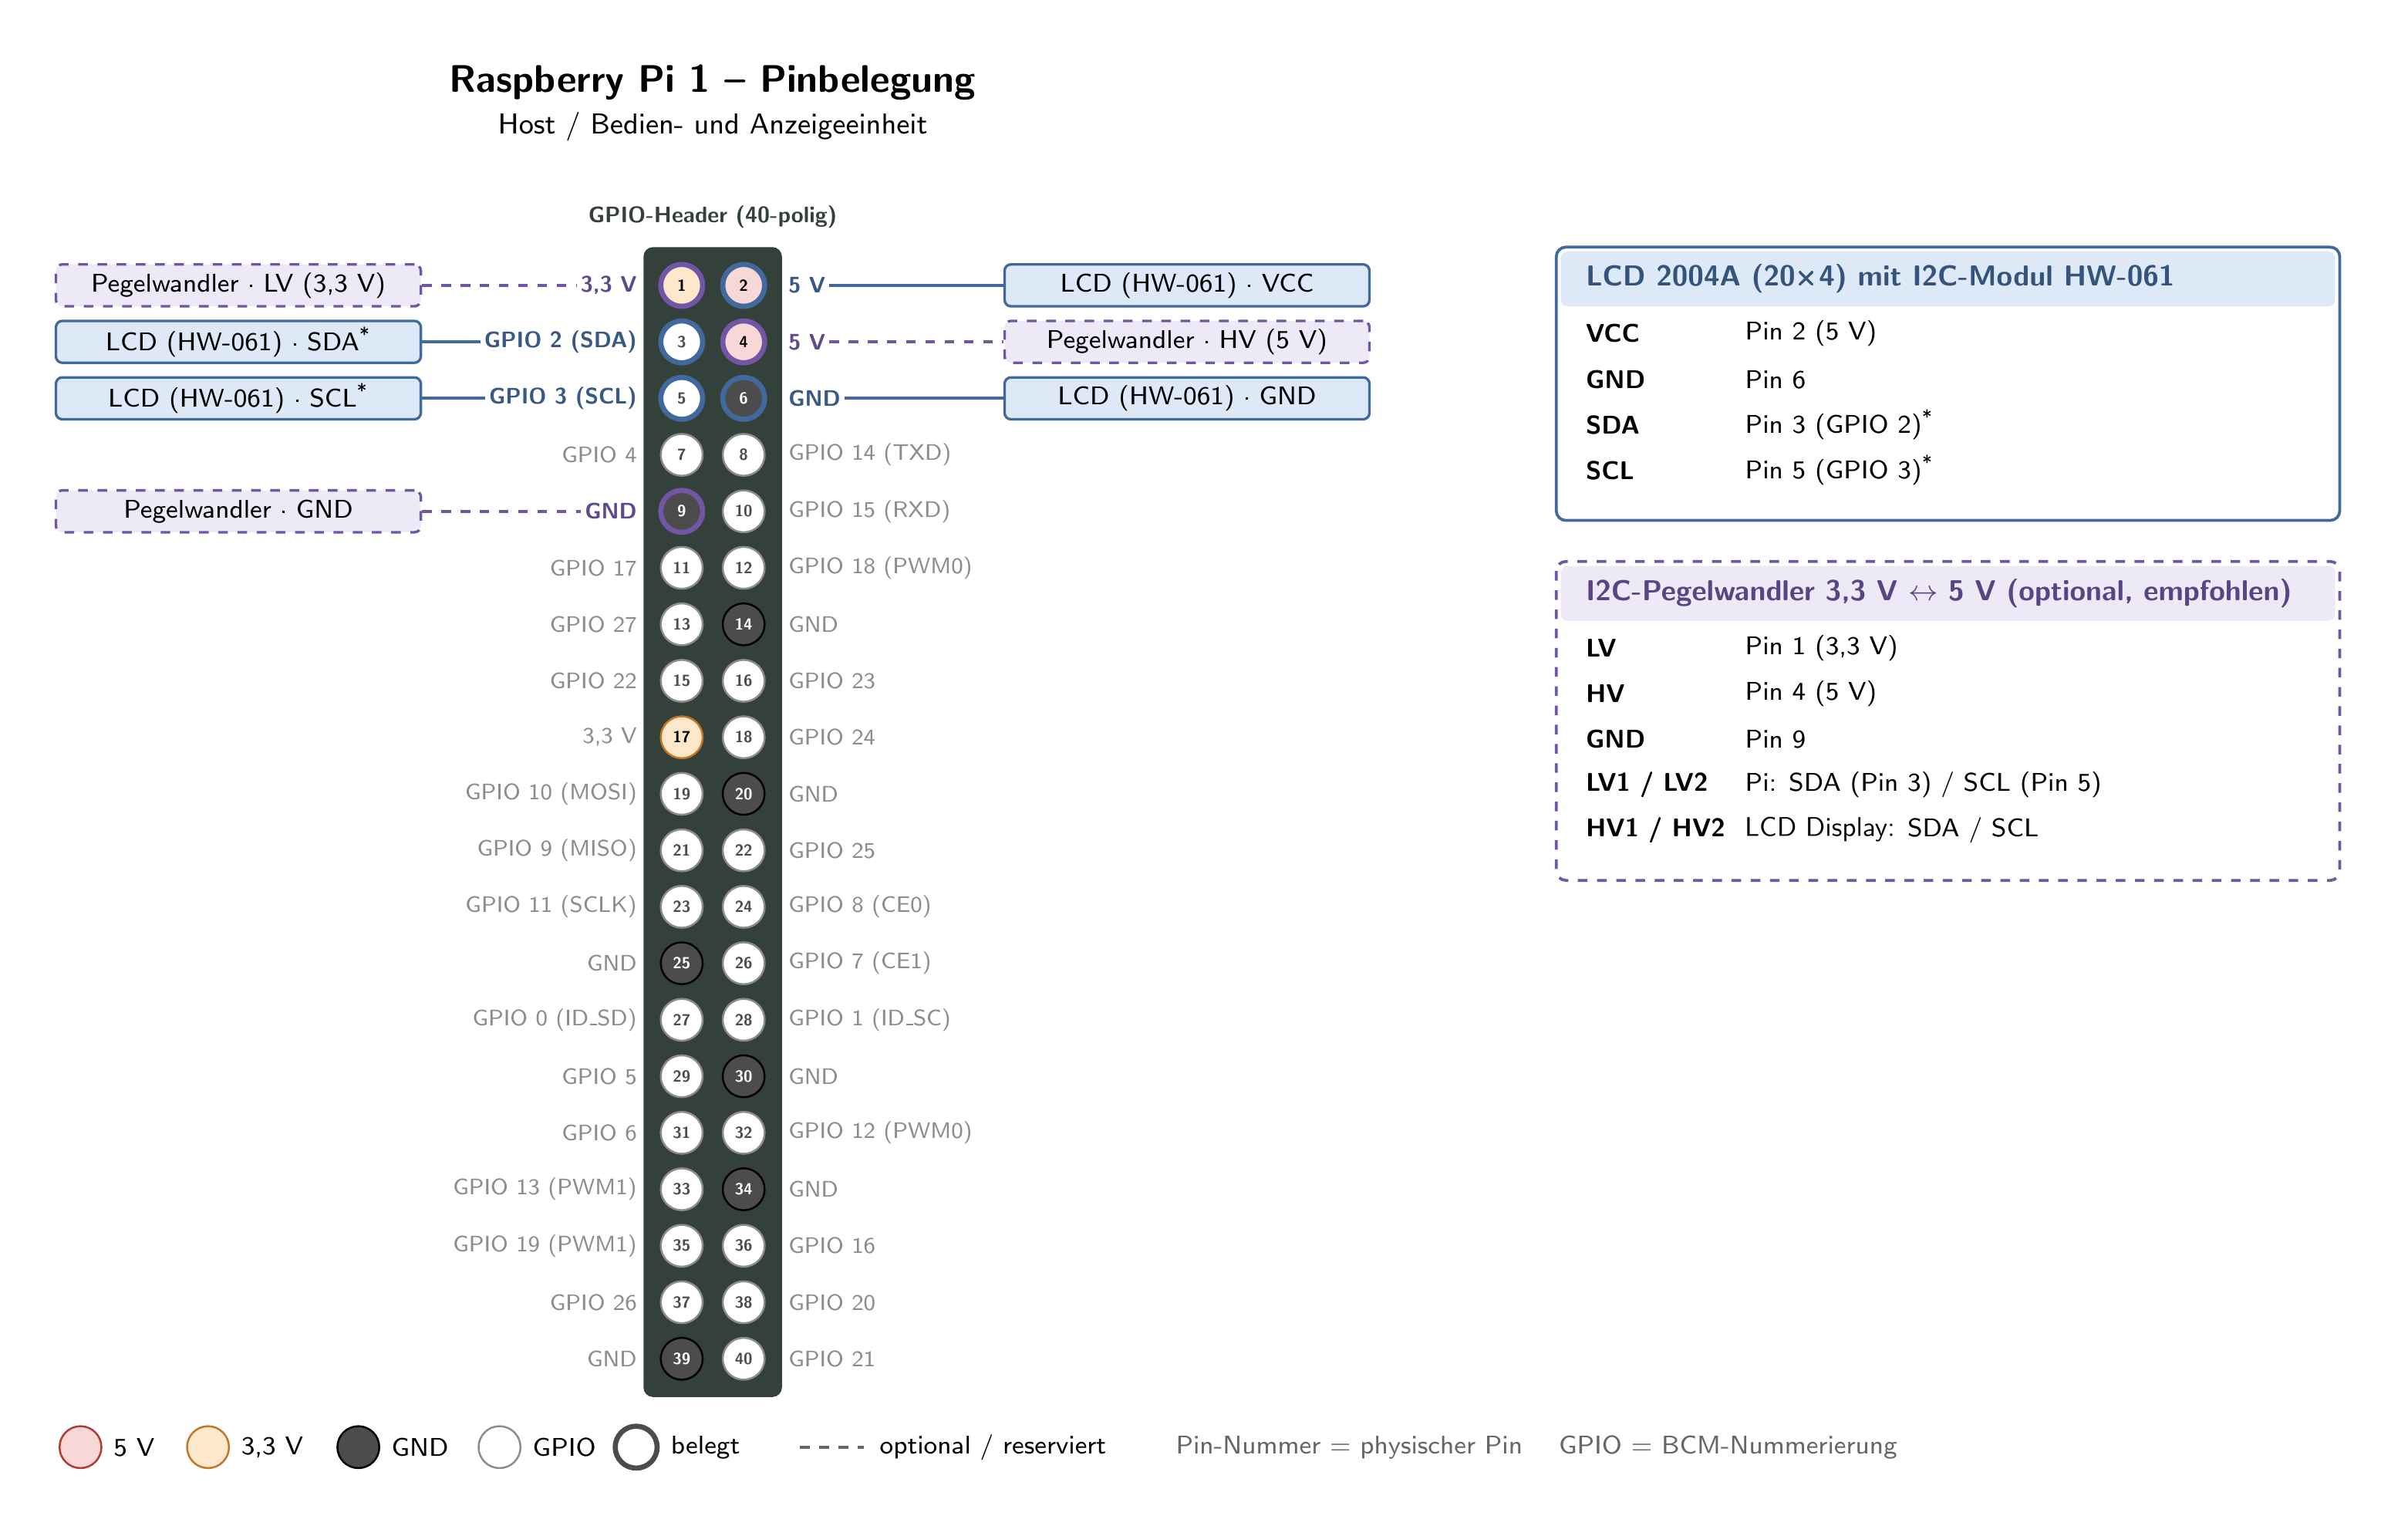
\includegraphics[width=0.8\textwidth]{images/pinout_pi1.png}
    \caption{Pinbelegung von Raspberry Pi 1}
    \label{fig:pinout_pi1}
\end{figure}

\begin{figure}[H]
    \centering
    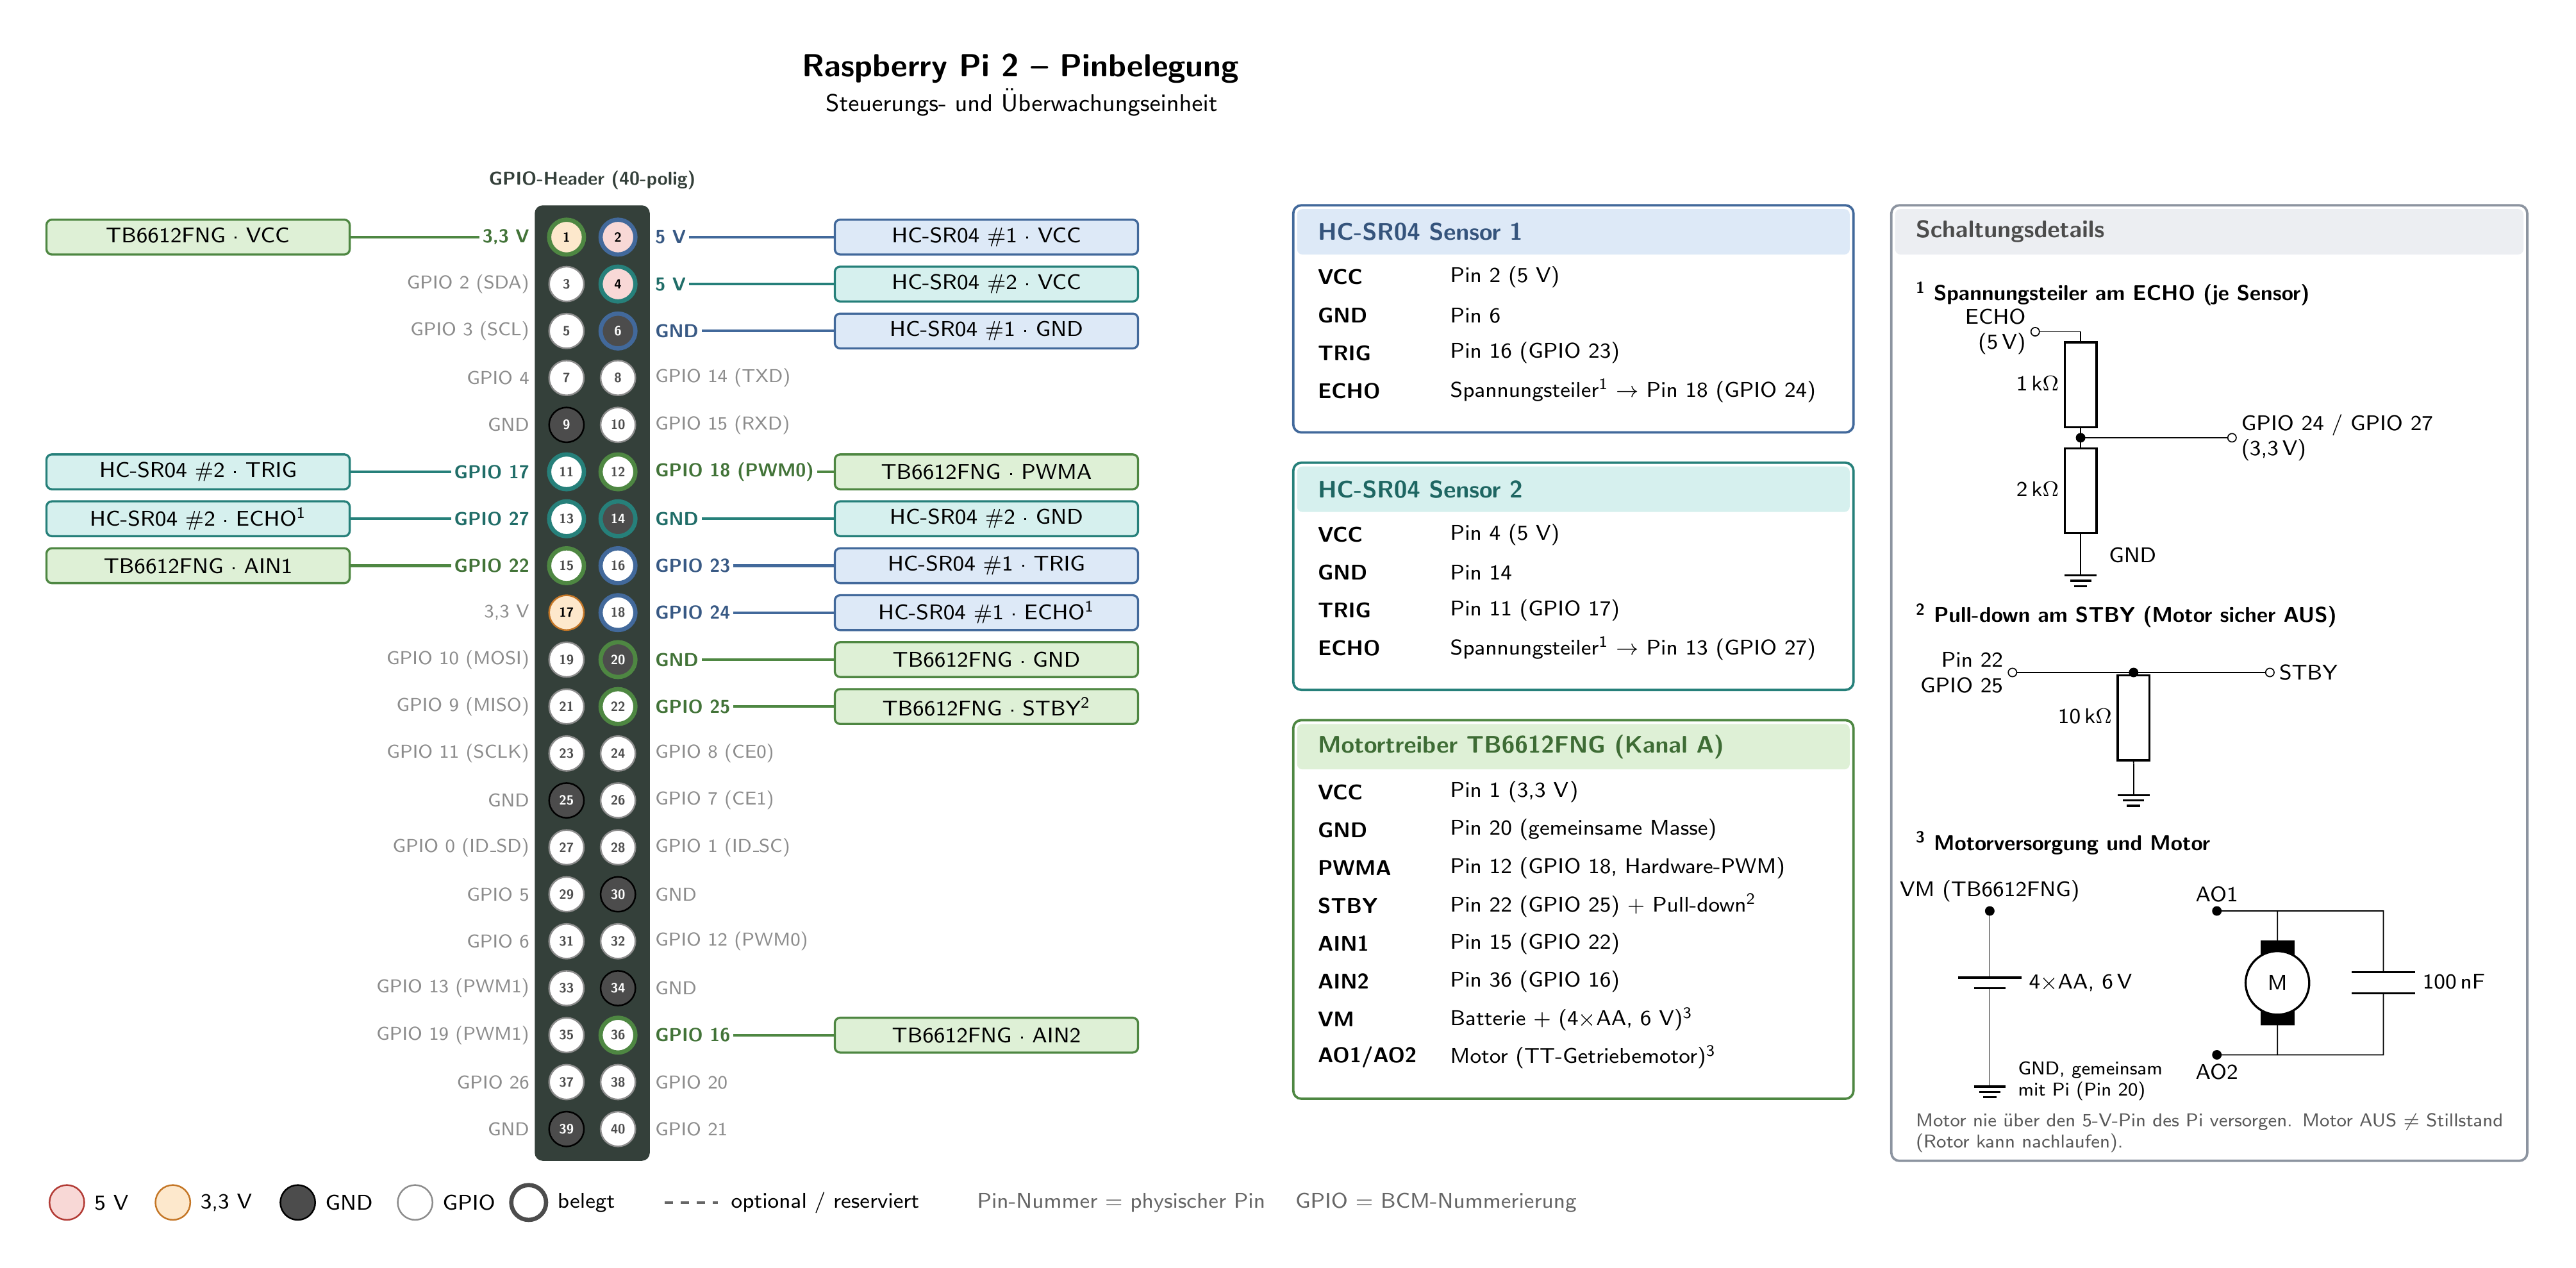
\includegraphics[width=0.8\textwidth]{images/pinout_pi2.png}
    \caption{Pinbelegung von Raspberry Pi 2}
    \label{fig:pinout_pi2}
\end{figure}
Der Link zum GitHub-Repository lautet \url{https://github.com/freudehcw/Safety_Strategies_Gruppe3}
